\documentclass[]{article}

\usepackage[margin=1.0in]{geometry}
\usepackage{amsmath}
\usepackage{amsfonts}
\usepackage{amsthm}
\usepackage{graphicx}
\usepackage{amssymb}

\usepackage{mathtools}

%opening
\title{Computing the Hausdorff Dimension for Symmetric Schottky Groups}
\author{Alex Karlovitz}
\date{}

\begin{document}
	
	\maketitle
	
\section*{Schottky Groups in the Unit Disk}

We can form a Schottky group in the unit disk as follows:
let $\mathcal{C}$ be a finite collection of disjoint circles which are orthogonal to the unit circle (actually, we will allow two circles in $\mathcal{C}$ to be tangent, so their intersections with the open unit disk are disjoint).
Then the group $\Gamma(\mathcal{C})$ generated by reflections across these circles in the unit disk is an example of a \textit{Schottky group}.

\subsection*{Example: Symmetric Circles}

A simple example of a Schottky group in the unit disk is obtained by taking circles of the same size spaced symmetrically about the disk.
We could parameterize such sets of circles by the two variables $n$ and $\theta$, where $n$ is the number of circles and $\theta$ is the angle along the unit circle cut out by one of the circles.
See Figure \ref{pi_over_2} for an example.

\begin{figure}[h]
	\centering
	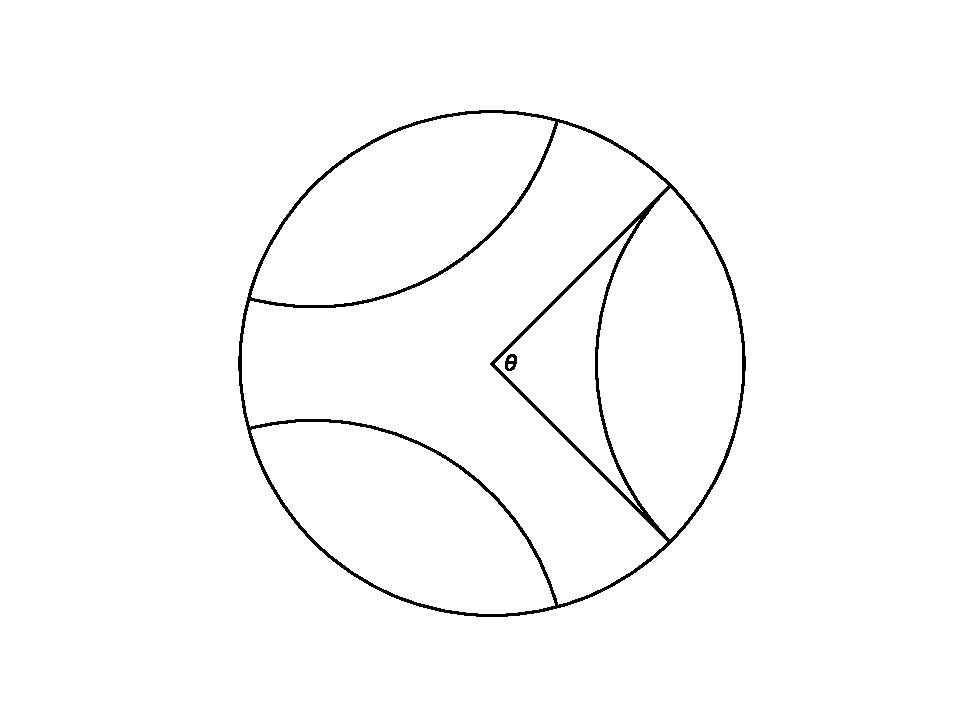
\includegraphics[trim=110 40 100 50, clip, width=0.6\linewidth]{pi_over_2.pdf}
	\caption{Example with $n = 3$ circles cutting out arcs of angle $\theta = \frac{\pi}{2}$}
	\label{pi_over_2}
\end{figure}

A fundamental domain for such a Schottky group is the exterior of all the circles (inside the unit disk of course).
To see this, label the reflections across the $n$ circles $R_1, \dots, R_n$.
We will also use $R_i$ to denote the actual reflections; the meaning should be clear from context.
Let
$$
\gamma = R_{i_1}\cdots R_{i_k}
$$
be a reduced word of length $k$ in the reflections (by \textit{reduced} we mean that $R_{i_j} \neq R_{i_{j+1}}$ for all $j$, since reflections are involutions).
Note that every element of the Schottky group can be written as such a reduced word.
Now suppose $z$ is any element of the fundamental domain.
If $k = 1$, then it is clear that $\gamma(z)$ is inside the circle $R_{i_1}$.
By induction, it is then easy to see that for $k \geq 1$, $\gamma(z)$ is always in the circle $R_{i_1}$.
Thus, the only way for $\gamma(z)$ to be in the fundamental domain is t o have $k = 0$; i.e., $\gamma$ is the identity.

To see that every orbit has a point in the fundamental domain, one must check that given a point in one of the circles $R_i$, reflection through that circle \textit{decreases} the distance from the point to $0$.
Thus, since the Schottky group acts discretely on hyperbolic space, we can eventually move any point to the fundamental domain by repeatedly reflecting outside of any circle it falls in.

See Figure \ref{disk_FD} for an example.

\begin{figure}[h]
	\centering
	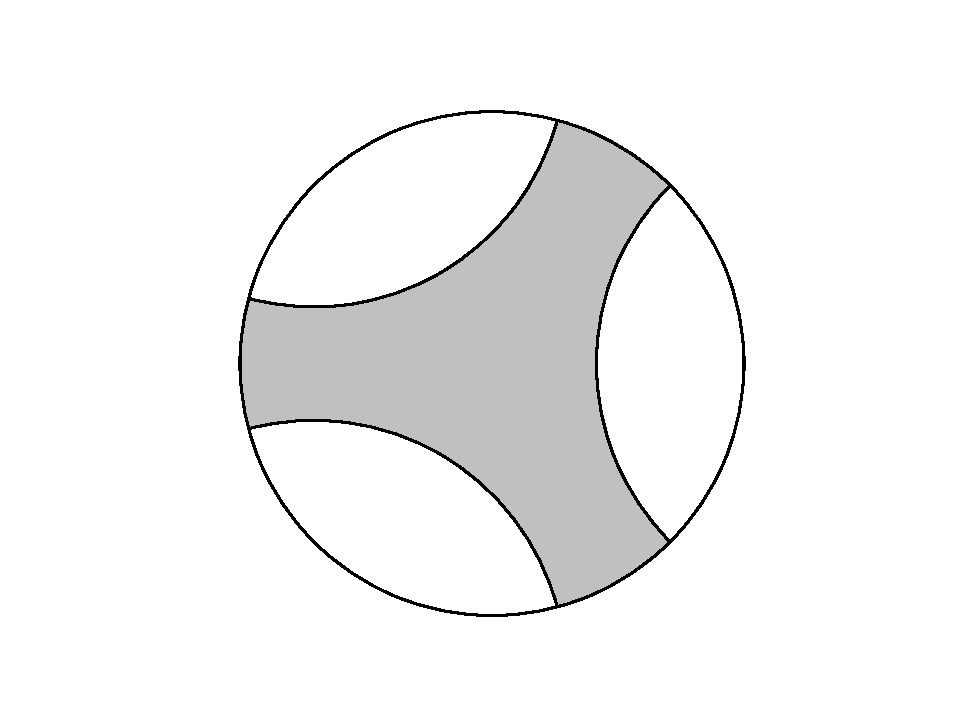
\includegraphics[trim=110 40 100 50, clip, width=0.6\linewidth]{disk_FD.pdf}
	\caption{The example from Figure \ref{pi_over_2} with a fundamental domain filled in.}
	\label{disk_FD}
\end{figure}

\textbf{Note:} For the rest of the document, we will focus on the case $n = 3$.
The discussion extends easily to $n > 3$.

\section*{Mapping to the Upper Half Plane}

Recall that we can map from the upper half plane model to the disk model via the \textit{Cayley transform}
$$
C(z) = \frac{z - i}{z + i}
$$
We can go the other direction by taking the inverse
$$
C^{-1}(w) = i\cdot\frac{1 + w}{1 - w}
$$
Also recall that $C$ and $C^{-1}$ send geodesics to geodesics.

Next, note that we are choosing to center one of our circles of reflection about $1$.
Since $C^{-1}(1) = \infty$, this has the effect of forcing our fundamental domain to be bounded inside $C^{-1}$ of that circle.
See Figure \ref{UHP_FD} for an example.

\begin{figure}[h]
	\centering
	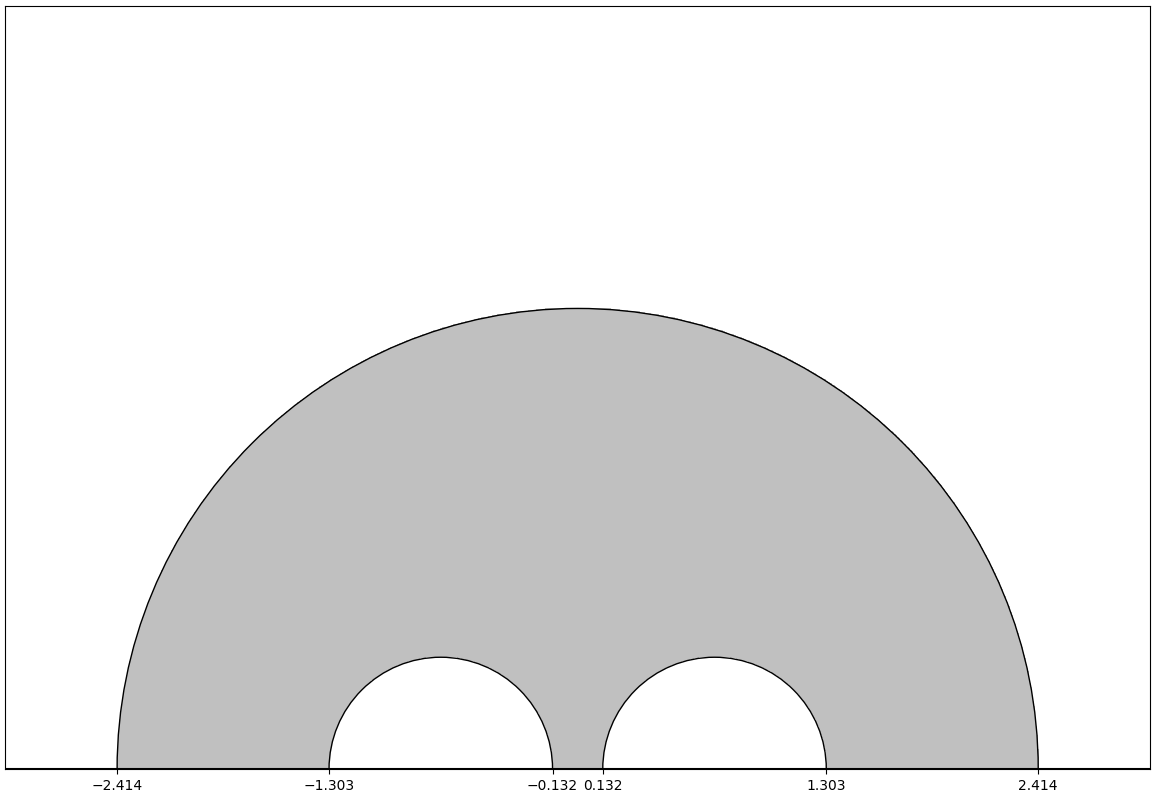
\includegraphics[width=0.6\linewidth]{UHP_FD.png}
	\caption{The example from Figure \ref{disk_FD} mapped to the upper half plane.}
	\label{UHP_FD}
\end{figure}

\textbf{Note:} this image seems to single out the middle flare as different from the other two, but this is just an artifact of our choice of Cayley transform.
We could just as easily have mapped $e^{\pi i/3}$ or $e^{-\pi i/3}$ to $-1$ instead.
\\

Finally, let's give a name to each of the circles involved.
In the disk, we will call the rightmost circle (which contains the point $1$) $R_1$.
We then proceed counterclockwise and name the next two circles $R_2$ and $R_3$.
The resulting labels in the upper half plane are shown in Figure \ref{UHP_labeled}.

\begin{figure}[h]
	\centering
	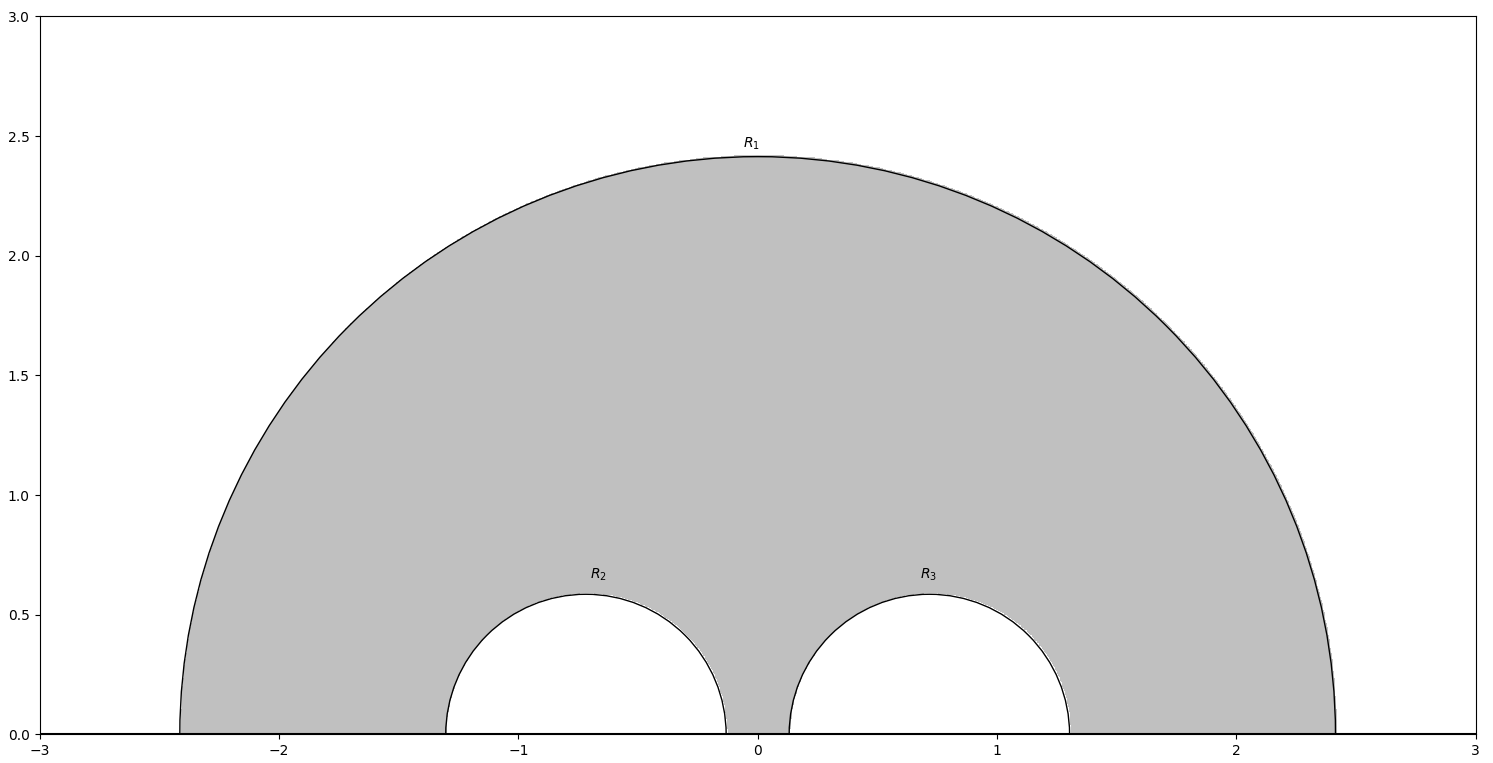
\includegraphics[width=0.6\linewidth]{UHP_labeled.png}
	\caption{Labeling of the circles from Figure \ref{UHP_FD}.}
	\label{UHP_labeled}
\end{figure}

\subsection*{Identifying Flare Domains}

Let us call the group generated by our three reflections
$$
\Gamma = \langle R_1, R_2, R_3 \rangle
$$
To get a flare domain, we need to identify a hyperbolic element in $\Gamma$ whose axis\footnote{Recall that the \textit{axis} of a hyperbolic matrix is the geodesic whose endpoints are the fixed points of the matrix.} ``cuts off'' a flare in our fundamental domain.
To do this, we first recall that even length words in circle reflections give M\"obius transformations.
Thus, we could look for appropriate hyperbolic matrices by checking small words of even length in our generators.
Indeed, one quickly finds that $R_1R_2, R_1R_3$, and $R_2R_3$ are hyperbolic matrices with appropriate axes (see Figure \ref{UHP_flares}).

\begin{figure}[h]
	\centering
	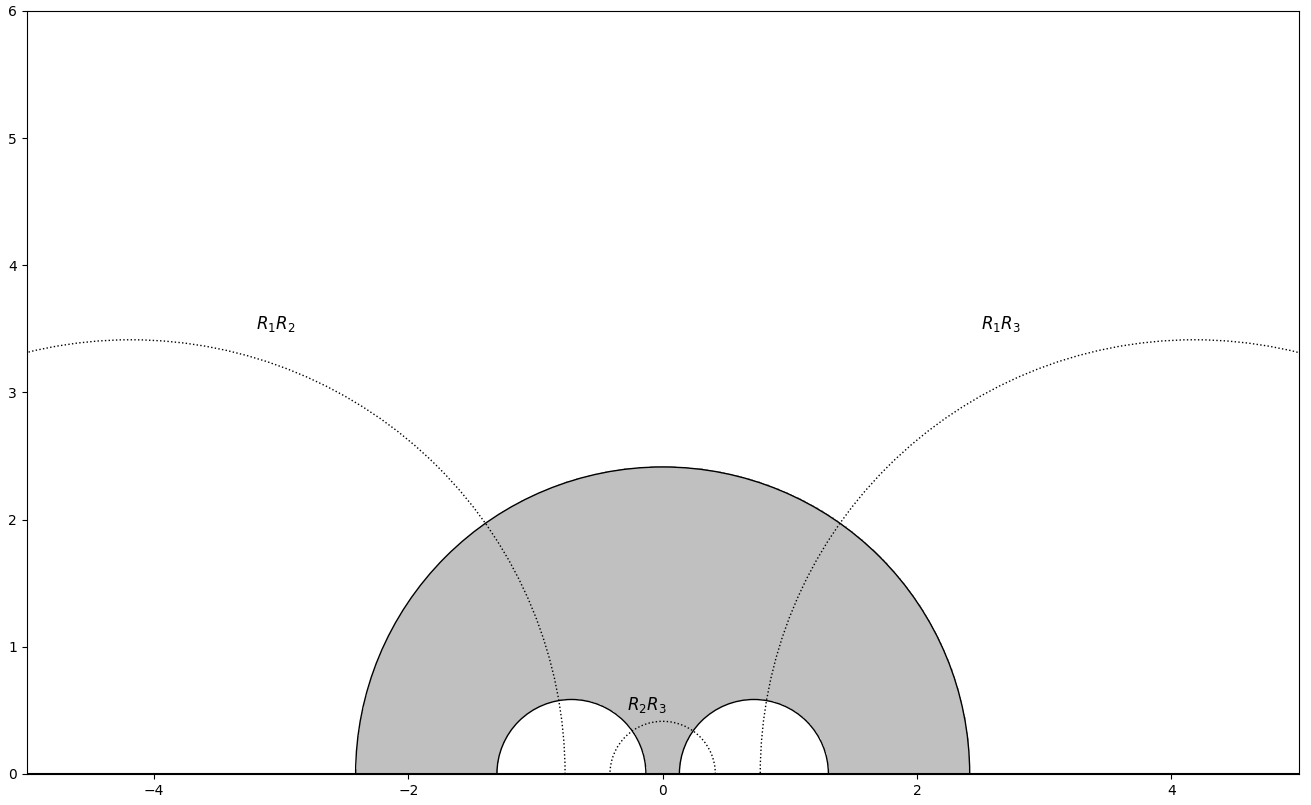
\includegraphics[width=0.6\linewidth]{UHP_flares.png}
	\caption{Axes cutting off flares labeled with the associated hyperbolic matrices.}
	\label{UHP_flares}
\end{figure}

Let's be a bit more formal in our discussion of flares.
To identify a flare between geodesics $C_1$ and $C_2$, one may look for a geodesic with the following properties:
\begin{itemize}
	\item one endpoint of the geodesic is on the other side of $C_1$ from the flare
	\item the other endpoint is on the other side of $C_2$ from the flare
	\item the geodesic meets $C_1$ and $C_2$ at right angles
\end{itemize}
In our situation, it is always possible to find a hyperbolic element in $\Gamma$ whose axis satisfies these properties.
To see this, one looks in inversive coordinates (see Kontorovich's letter to Bill Duke).
Letting $v_1$ and $v_2$ denote the inversive coordinates for $C_1$ and $C_2$, respectively, one looks for the inversive coordinates $v$ such that
$$
v_1^tQv = 0 ~~~~~ v_2^tQv = 0 ~~~~~ v^tQv = -1
$$
where $Q$ is the quadratic form defining inversive coordinates.
The first two equations give the orthogonality, and the third gives a true vector of inversive coordinates.
Finally, these coordinates give the endpoints of our geodesic.
To find the corresponding M\"obius transformation in $\Gamma$, one searches over all transformations with this axis for the one taking the intersection point with $C_1$ to that of $C_2$.

\clearpage

\section*{Mapping to a Flare Domain}

Let us look at a generic flare: two geodesics separated by positive length interval on the real line, plus a geodesic cutting through both of these at a right angle.
Let the two points on this last geodesic be labeled $z_1 < z_2$, and call the rightmost point of the first geodesic $t$.
See Figure \ref{pre_flare}.
\begin{figure}[h]
	\centering
	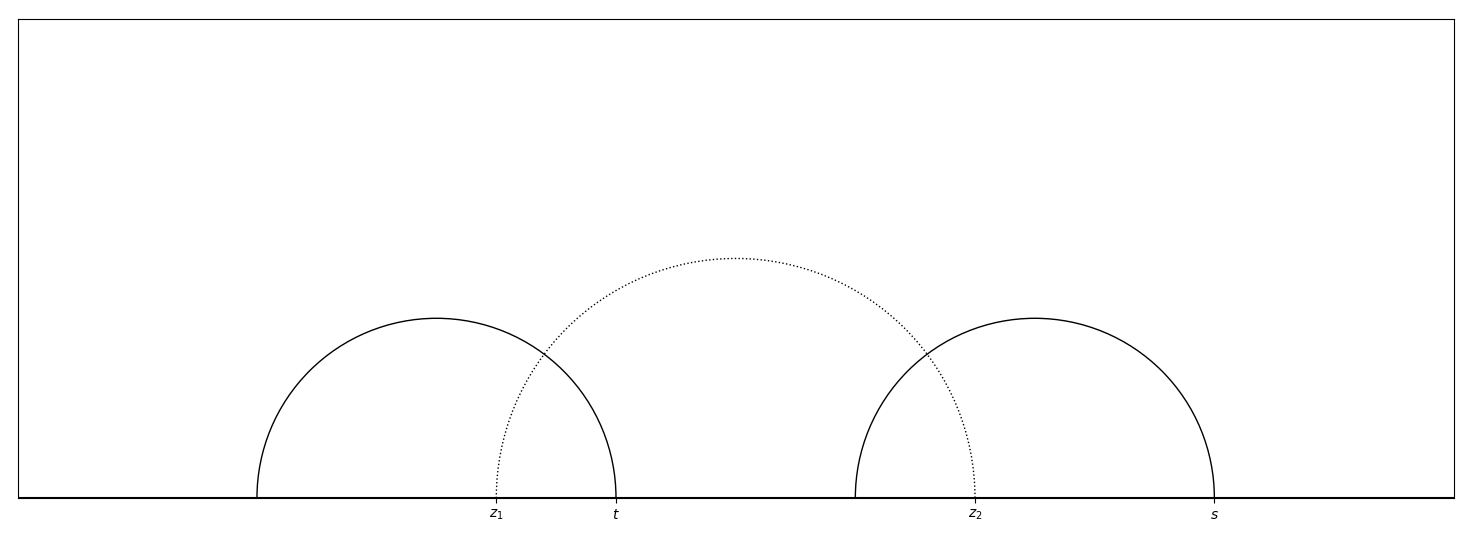
\includegraphics[width=0.6\linewidth]{labeled_pre_flare.png}
	\caption{A generic flare.}
	\label{pre_flare}
\end{figure}
Now consider the M\"obius transformation
$$
U(z) = \left( \frac{t - z_2}{t - z_1} \right) \frac{z - z_1}{z - z_2}
$$
This function is chosen so that
$$
U(z_1) = 0 ~~~~~ U(z_2) = \infty ~~~~~ U(t) = 1
$$
Thus, applying such a $U$ to a generic flare gives us a \textit{flare domain}.
See Figure \ref{post_flare} for an example.
\begin{figure}[h]
	\centering
	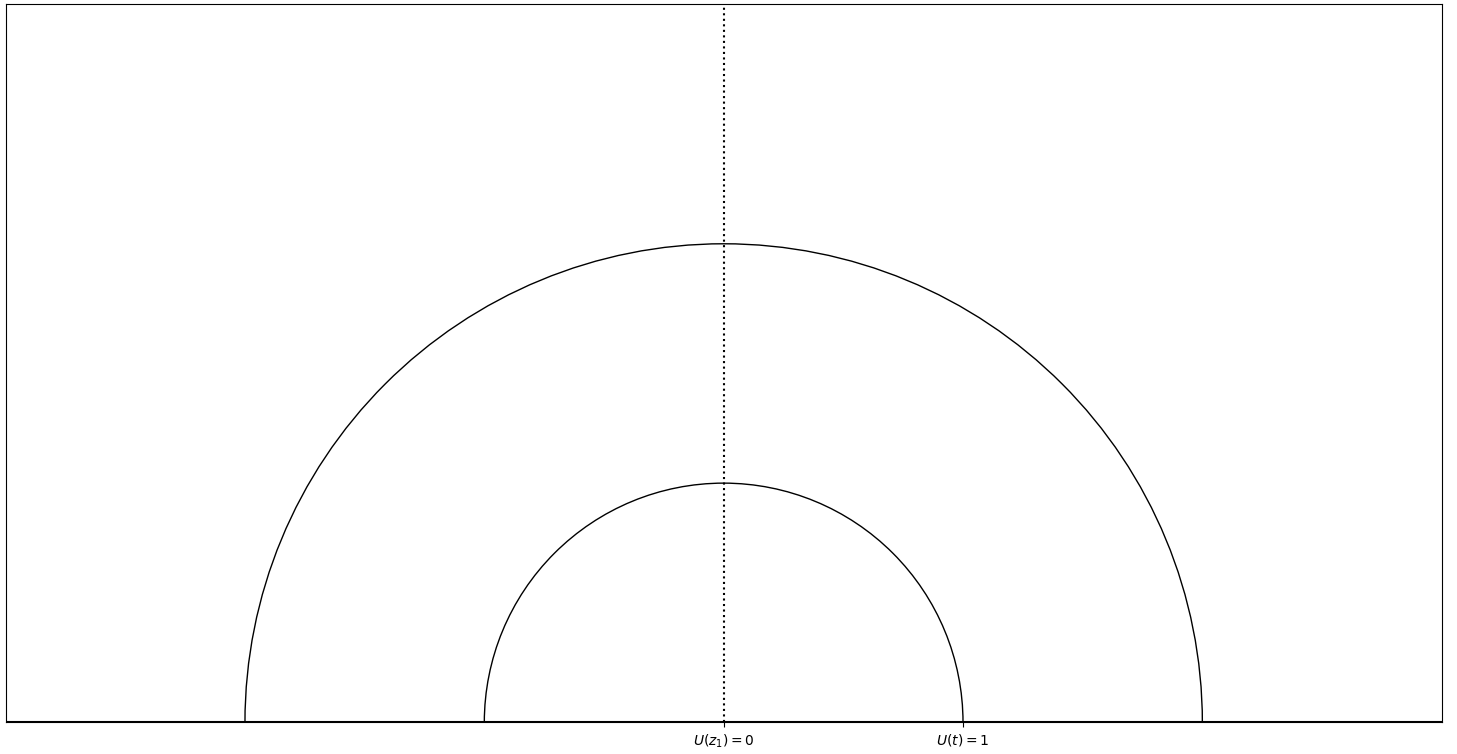
\includegraphics[width=0.6\linewidth]{labeled_flare.png}
	\caption{A flare domain.}
	\label{post_flare}
\end{figure}

Let's consider our symmetric Schottky group example.
Using the flare cut off by the axis of $R_2R_3$, we get the flare domain pictured in Figure \ref{flare}.
\begin{figure}[h]
	\centering
	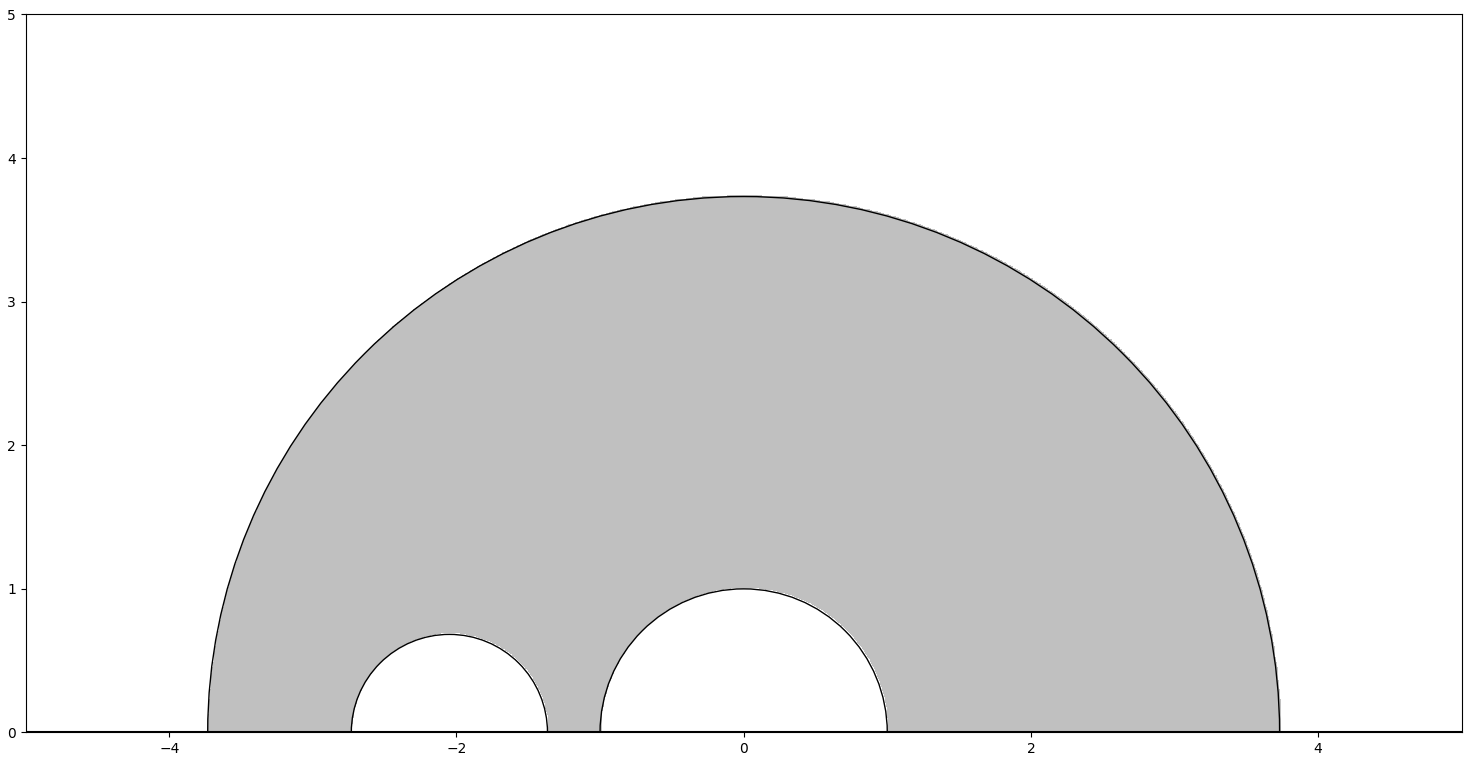
\includegraphics[width=0.6\linewidth]{flare.png}
	\caption{The flare domain obtained from middle flare in Figure \ref{UHP_flares}.}
	\label{flare}
\end{figure}

\clearpage

\section*{Rotational Symmetry of Maass Forms}

Recall that Maass forms for $\Gamma$ are eigenfunctions of the Laplace-Beltrami operator acting on $L^2(\Gamma\backslash\mathbb{H})$.
We claim that for a given eigenvalue, a Maass form for the symmetric Schottky group of parameters $(n, \theta)$ can be taken to be invariant under rotation by $2\pi/n$.
\\

To verify this claim, first recall that the Laplace operator on the disk model (in polar coordinates) is
$$
\Delta = -\left(\frac{(1 - \rho^2)^2}{4}\frac{\partial^2}{\partial\rho^2} +
\frac{(1 - \rho^2)^2}{4\rho}\frac{\partial}{\partial\rho} +
\frac{(1 - \rho^2)^2}{4\rho^2}\frac{\partial^2}{\partial\theta^2}\right)
$$
From this formula, one easily sees that rotations are $\Delta$-invariant.
Thus, if we compose any eigenfunction of the Laplacian with a rotation, we still have an eigenfunction of the same eigenvalue.

Next, note that a rotation of $2\pi/n$ is smooth on the fundamental domain for the $(n, \theta)$ symmetric Schottky group.
Thus, given a Maass form $f$, we can construct a $2\pi/n$ rotation-invariant Maass form of the same eigenvalue by taking the linear combination
$$
\frac{1}{n}\sum_{i = 0}^{n - 1}f\left(e^{2\pi i/n} z\right)
$$

So we can assume that any Maass form we are working with is invariant under rotation by $2\pi/n$.
Even further, we can use the multiplicity one principle to conclude that the base eigenfunction is itself invariant under this rotation.

\subsection*{Consequences for Hejhal's Algorithm}

When running Hejhal's algorithm on the symmetric Schottky groups, we need only consider test points in one $2\pi/n$ sector.
We can of course take this sector to entirely contain one flare, while not intersecting any others.

If the pullback $z^*$ of a test point $z$ falls outside of the chosen sector, we can simply replace $z^*$ with the appropriate rotation to make it fall in this sector, since the Maass form will be equivalent at those different points.

\end{document}